\section{Computer Vision}

\subsection{Camera Geometry (10 marks)}

$f = \SI{10}{\mm}$

$D = \SI{10}{\m} = \SI{10000}{\mm}$

$sensor: \SI{10}{\mm} \times \SI{10}{\mm} = 1000 \times 1000 \text{ pixels}$

$h = 100 \text{ pixels} = \SI{1}{\mm}$

\begin{multicols}{2}

\begin{align*}
    \frac{1}{D} + \frac{1}{d} &= \frac{1}{f} \\[1.25ex]
    \frac{1}{d} &= \frac{1}{f} - \frac{1}{D} \\[1.25ex]
    \frac{1}{d} &= \frac{1}{10} - \frac{1}{10000} \\[1.25ex]
    \frac{1}{d} &= \frac{1000}{10000} - \frac{1}{10000} \\[1.25ex]
    \frac{1}{d} &= \frac{999}{10000} \\[1.25ex]
    d &= \frac{10000}{999}
\end{align*}

\begin{align*}
    \frac{d}{D} &= \frac{h}{H} \\[1.25ex]
    H &= \frac{hD}{d} \\[1.25ex]
    H &= \frac{1 \times 10000}{\cfrac{10000}{999}} \\[1.25ex]
    H &= \SI{999}{\mm} = \SI{0.999}{\m}
\end{align*}

\end{multicols}

The observed statue is \SI{0.999}{\m} tall.

\bigskip

\begin{center}
\begin{tikzpicture}

    % horizon
    \draw[dashed] (0, 0) -- (0.82\textwidth, 0);

    % statue image
    \node[inner sep=0pt] (statue) at (1, 0.15\textwidth)
        {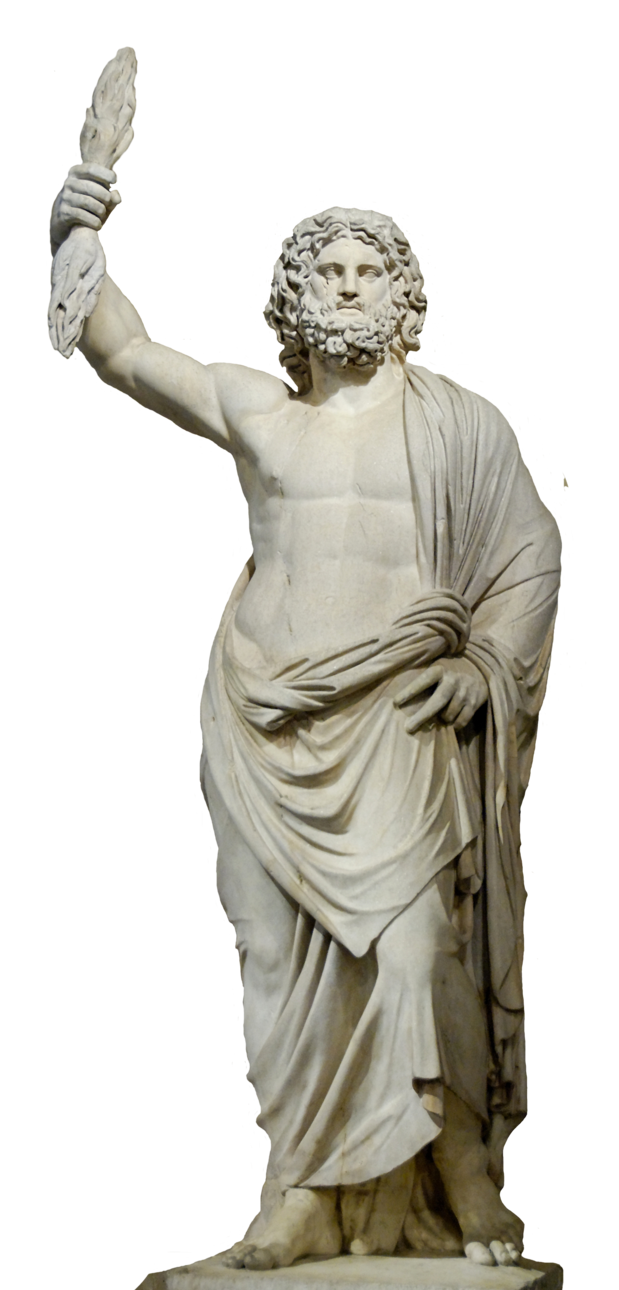
\includegraphics[height=0.3\textwidth]{res/statue.png}};

    % lens
    \draw (0.7\textwidth, 0) ellipse (1mm and 3mm);

    % film
    \draw (0.79\textwidth, -1) rectangle (0.8\textwidth, 1);

    % statue projection
    \draw (statue.north) -- (0.79\textwidth, -0.5);

    % H
    \draw[thick, <->] (statue.south west) -- (statue.north west) node[midway, anchor=east] {H};

    % D
    \draw[thick, <->] (1, -0.8) -- (0.7\textwidth, -0.8) node[midway, anchor=north] {D};

    % d
    \draw[thick, <->] (0.7\textwidth, -0.8) -- (0.79\textwidth, -0.8) node[midway, anchor=north] {d};

    % h
    \draw[thick, <->] (0.81\textwidth, 0) -- (0.81\textwidth, -0.5) node[midway, anchor=west] {h};

\end{tikzpicture}
\end{center}

\bigskip

The distance $D$ to the statue needs to be known in order to calculate the distance $d$ between the lens and the film/sensor, using the focal length $f$. Furthermore, given $D$, $d$, and $h$, it is easy to calculate the height of the statue $H$.

\clearpage

% - - - - - - - - - - - - - - - - - - - - - - - - - - -

\subsection{Image Processing (10 marks)}

The following row of images/samples is a visual representation of the \textit{intermediate} keypoints of the car counter program.

\begin{center}
    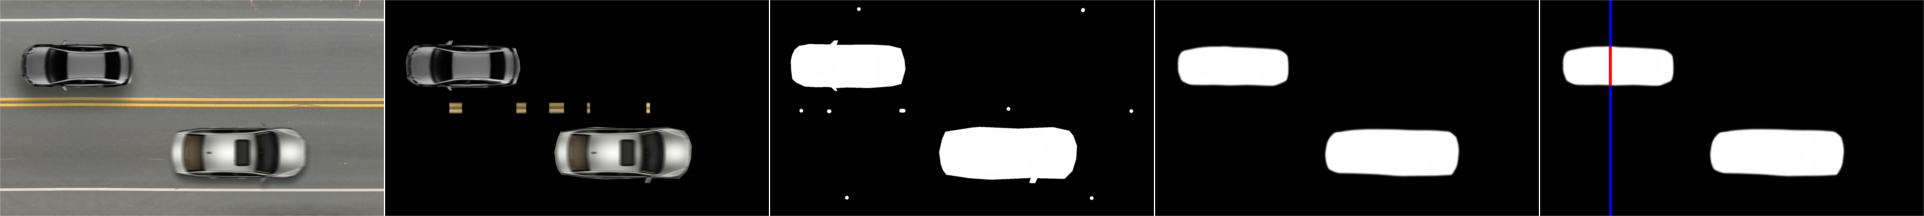
\includegraphics[width=\textwidth]{res/32.png}
\end{center}

Firstly the program fetches the frames from the live camera feed - the first image from the row of images above is an example of a frame fetched from the camera.\\
Afterwards it does a \textit{image segmentation} by applying a \textit{background removal} technique - second image, counting from the left, in the images row above.\\
At this point it is useful to turn the image into a binary image - middle image sample.\\
Then two \textit{morphological transformations} are applied to remove the noise left in the frame - also known as \textit{morphological closing} and \textit{opening} - penultimate image sample.\\
Finally the last image from the samples row above shows the \textit{region of interest} - region in blue, activated by the passing car (red segment of the detection region).

The general idea is to count every time a white spot is detected in the blue line - actually, to introduce some tolerance, it should not be a line with a single pixel thickness, rather a 5 pixels thick line, for example.

Furthermore, to save computation time, and since we only care for what is going on inside the blue region, we can \textit{crop} everything else besides that region right after the frame capture. Nonetheless, the entire frame of each of the samples above is used (no cropping) for better understanding of the main idea.

\begin{algorithm}
    \caption{Car counter program}\label{carCounterProg}
    \begin{algorithmic}[1]
        \Procedure{CarCounter}{}
            \State $ carPassing \leftarrow \texttt{False} $
            \State $ carCounter \leftarrow 0 $
            \Loop
                \State $ frame \leftarrow cam.fetchFrame() $
                \State $ CropRegionOfInterest(frame) $ \Comment{Crop to save computation time}
                \State $ SubtractBg(frame) $
                \State $ BinaryThreshold(frame) $
                \State $ MorphOpen(frame) $
                \State $ MorphClose(frame) $
                \If{$ carFound(frame) $}
                    \If{$ \texttt{not } carPassing $}
                        \State $ carPassing \leftarrow \texttt{True} $
                        \State $ counter \leftarrow counter + 1 $
                    \EndIf
                \ElsIf{carPassing}
                    \State $ carPassing \leftarrow \texttt{False} $
                \EndIf
            \EndLoop
        \EndProcedure

        \Statex

        \Function {SubtractBg}{$ frame $}
            \State $ hourOfDay \leftarrow getTime().hour $
            \State $ bg \leftarrow DB.image(\text{"backgrounds/"} + hourOfDay + \text{".png"}) $
            \State $ frame.subtractImg(bg) $
        \EndFunction

        \Statex

        \Function {MorphOpen}{$ frame $}
            \State erode(frame)
            \State dillate(frame)
        \EndFunction

        \Statex

        \Function {MorphClose}{$ frame $}
            \State dillate(frame)
            \State erode(frame)
        \EndFunction

        \Statex

        \Function {CarFound}{$ frame $}
            \For{$ i \gets 0, frame.size $}
                \For{$ j \gets 0, frame[i].size $}
                    \If{$ frame[i][j] = RGB(255, 255, 255) $}
                        \State \textbf{return} $ \texttt{True} $
                    \EndIf
                \EndFor
            \EndFor
            \State \textbf{return} $ \texttt{False} $
        \EndFunction
    \end{algorithmic}
\end{algorithm}

\clearpage

% - - - - - - - - - - - - - - - - - - - - - - - - - - -

\subsection{Shape Recognition (10 marks)}

The first thing to do in order to narrow the search results by 50\% is to check if the card has \textit{red} or \textit{black} symbols - a simple \textit{RGB normalization} can be used. After this step the search results are narrowed either to \textit{spades and clubs}, or \textit{hearts and diamonds}.

A Bayes classifier needs to be trained using \textit{4 classes}, one for each suit.

\newpage
